% Created 2021-09-27 Mon 12:01
% Intended LaTeX compiler: xelatex
\documentclass[letterpaper]{article}
\usepackage{graphicx}
\usepackage{grffile}
\usepackage{longtable}
\usepackage{wrapfig}
\usepackage{rotating}
\usepackage[normalem]{ulem}
\usepackage{amsmath}
\usepackage{textcomp}
\usepackage{amssymb}
\usepackage{capt-of}
\usepackage{hyperref}
\setlength{\parindent}{0pt}
\usepackage[margin=1in]{geometry}
\usepackage{fontspec}
\usepackage{svg}
\usepackage{cancel}
\usepackage{indentfirst}
\setmainfont[ItalicFont = LiberationSans-Italic, BoldFont = LiberationSans-Bold, BoldItalicFont = LiberationSans-BoldItalic]{LiberationSans}
\newfontfamily\NHLight[ItalicFont = LiberationSansNarrow-Italic, BoldFont       = LiberationSansNarrow-Bold, BoldItalicFont = LiberationSansNarrow-BoldItalic]{LiberationSansNarrow}
\newcommand\textrmlf[1]{{\NHLight#1}}
\newcommand\textitlf[1]{{\NHLight\itshape#1}}
\let\textbflf\textrm
\newcommand\textulf[1]{{\NHLight\bfseries#1}}
\newcommand\textuitlf[1]{{\NHLight\bfseries\itshape#1}}
\usepackage{fancyhdr}
\pagestyle{fancy}
\usepackage{titlesec}
\usepackage{titling}
\makeatletter
\lhead{\textbf{\@title}}
\makeatother
\rhead{\textrmlf{Compiled} \today}
\lfoot{\theauthor\ \textbullet \ \textbf{2021-2022}}
\cfoot{}
\rfoot{\textrmlf{Page} \thepage}
\renewcommand{\tableofcontents}{}
\titleformat{\section} {\Large} {\textrmlf{\thesection} {|}} {0.3em} {\textbf}
\titleformat{\subsection} {\large} {\textrmlf{\thesubsection} {|}} {0.2em} {\textbf}
\titleformat{\subsubsection} {\large} {\textrmlf{\thesubsubsection} {|}} {0.1em} {\textbf}
\setlength{\parskip}{0.45em}
\renewcommand\maketitle{}
\author{Houjun Liu}
\date{\today}
\title{The Cell Cycle}
\hypersetup{
 pdfauthor={Houjun Liu},
 pdftitle={The Cell Cycle},
 pdfkeywords={},
 pdfsubject={},
 pdfcreator={Emacs 28.0.50 (Org mode 9.4.4)}, 
 pdflang={English}}
\begin{document}

\tableofcontents



\section{The Cell Cycle}
\label{sec:org663ab03}
The cell cycle is roughly three parts which is really 5 parts which is
really 9 parts.

The three main parts are:

\begin{itemize}
\item \textbf{Interphase} --- G1, S, G2: systems preperation for mitosis
\item \textbf{Mitosis} --- Separation of the duplicated chromosomes
\item \textbf{Cytokinesis} --- the splitting of the cell itself. Really part of
mitosis
\end{itemize}

\subsection{Features of the Cell Cycle}
\label{sec:orga0676b7}
\textbf{\emph{Most} cell division results in genetically identical daughter cell}

Each cell, once specialised, chooses what parts of their chromasome to
unwrap + permanently wrap.

Difference in transcription results in different phenotypes.

Sperm + Egg (imcomplete cells) combine together to form a "zygote" => a
single cell. Each person is from a zygote.

\href{https://docs.google.com/document/d/1TIrgR9VSV3attTK\_QP-AOCs33mMoBP0Cz7DQXysKoD0/edit}{Paul's
Cell Cycle Primer}

\begin{figure}[htbp]
\centering
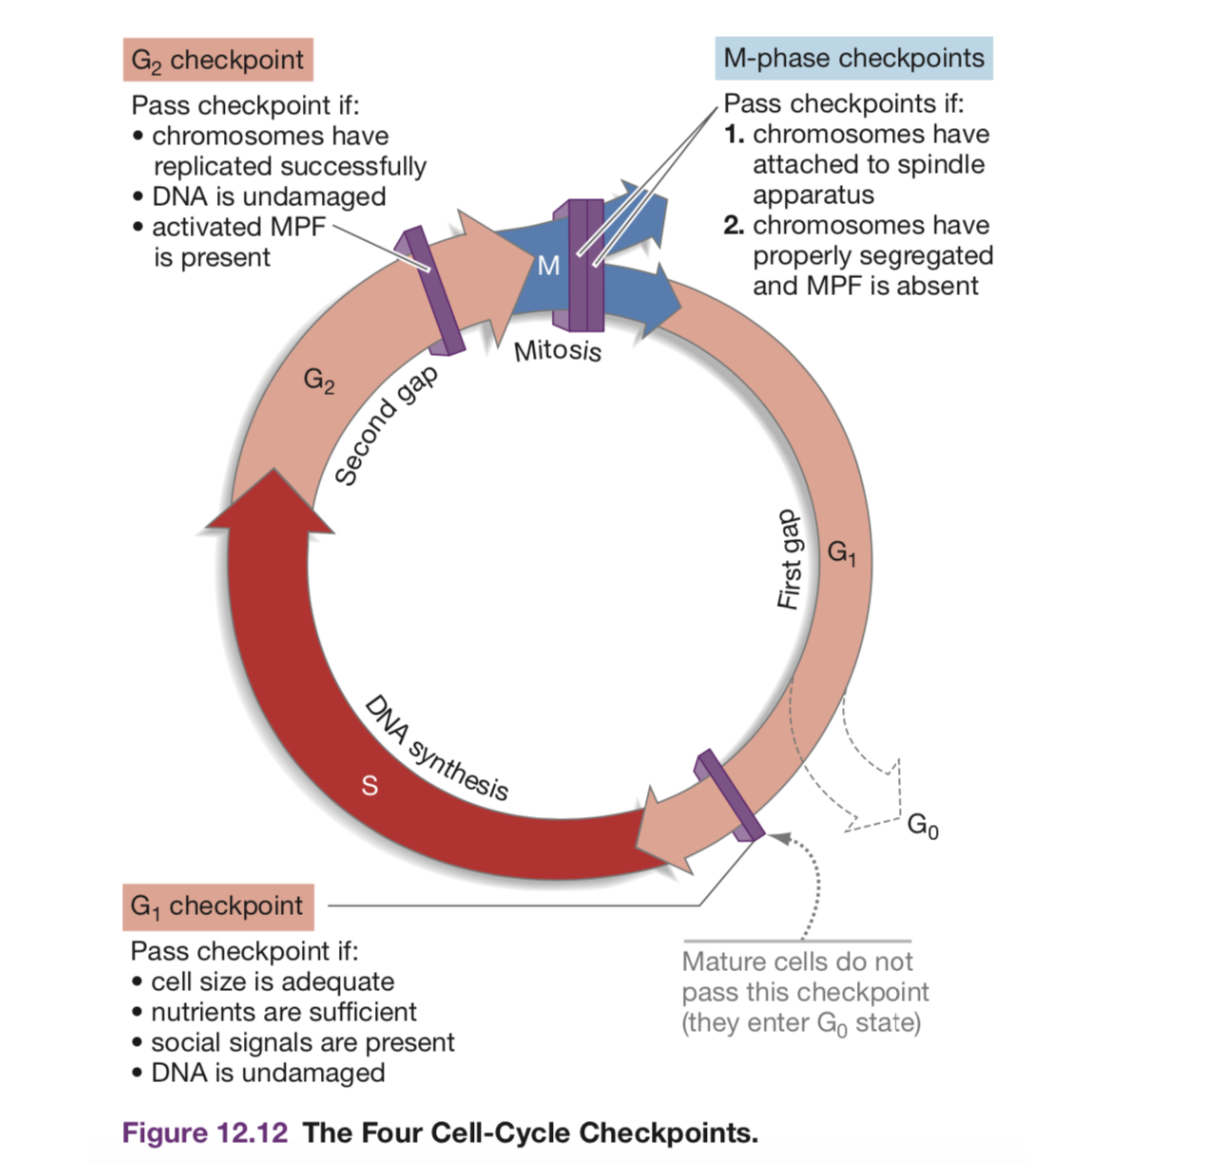
\includegraphics[width=.9\linewidth]{Screen Shot 2020-11-09 at 3.16.12 PM.png}
\caption{Screen Shot 2020-11-09 at 3.16.12 PM.png}
\end{figure}

\subsection{The Phrases}
\label{sec:org230406b}
\subsubsection{G1 => Rest Phase, Gap 1}
\label{sec:orga697aef}
This is the phase which is the "daily life of a cell". There are two
major checkpoints in this phase which, upon it is reached, sets the rest
of the cell cycle into motion.

\begin{itemize}
\item May hit s.a. to volume checkpoint => if ratio too big, the cell is too
big
\item May hit diffusion checkpoint => larger cells would need to work harder
to transport things to the centre
\end{itemize}

At this phase, the organelles in the cytoplasm also replicates in
preparation for the S phase.

\subsubsection{S => S Phase, duplicate DNA. 150 mins}
\label{sec:org8298669}
In this process, all of the DNA that is in the nucleus will be
\href{KBhBIO101DNAReplication.org}{KBhBIO101DNAReplication}ed in order
to actually split the cell in half.

\subsubsection{G2 => Rest Phrase, Gap 2.}
\label{sec:org842d6d8}
The pairs of DNA begins bundling and condensing; the DNA is also checked
upon and verified for consistency and dumped based the needs of the
cell.

At this point, the enzymes needed to assist Mitosis is also synthesized.

\subsubsection{M => Mitosis!}
\label{sec:org1c9c258}
Mitosis is the process by which non-sex (somatic) cells actually divide.
It consists of four parts --- prophase, metaphase, anaphase, telophase
--- and a final seperation called cytokenisis. See
\href{KBhBIO101Mitosis.org}{KBhBIO101Mitosis}.

\textbf{or\ldots{}}

\subsubsection{M => Meiosis!}
\label{sec:org034c314}
Mitosis is the process by which sex cells (gametes) divide. It consists
of four parts --- prophase, metaphase, anaphase, telophase --- and
cytokinesis but TWICE! This process also has clever mechanisms to ensure
genetic diversity. See yourself:
\href{KBhBIO101Meiosis.org}{KBhBIO101Meiosis}

\subsection{Cell cycle regulation}
\label{sec:orgd9c9905}
Purpose of regulation: \textbf{Cells must meet certain conditions before moving
onto the next phase.}

Cell regulators are proteins that manage and sheperard the process of
cell division. They respond to molecular signals throughout the cell and
check for internal signals like DNA damage to control the rate and
progress of cell division.

See
\href{KBhBIO101CellCycleRegulation.org}{KBhBIO101CellCycleRegulation}

\subsection{How about Meiosis?}
\label{sec:org3b1d936}
\href{KBhBIO101Meiosis.org}{KBhBIO101Meiosis}  
\end{document}
